
\documentclass[journal,10pt,draftclsnofoot,onecolumn]{IEEEtran}

\usepackage{url}
% *** MISC UTILITY PACKAGES ***
%\usepackage{ifpdf}
% Heiko Oberdiek's ifpdf.sty is very useful if you need conditional
% compilation based on whether the output is pdf or dvi.
% usage:
% \ifpdf
%   % pdf code
% \else
%   % dvi code
% \fi
% The latest version of ifpdf.sty can be obtained from:
% http://www.ctan.org/tex-archive/macros/latex/contrib/oberdiek/
% Also, note that IEEEtran.cls V1.7 and later provides a builtin
% \ifCLASSINFOpdf conditional that works the same way.
% When switching from latex to pdflatex and vice-versa, the compiler may
% have to be run twice to clear warning/error messages.

% *** CITATION PACKAGES ***
%
%\usepackage{cite}
% cite.sty was written by Donald Arseneau
% V1.6 and later of IEEEtran pre-defines the format of the cite.sty package
% \cite{} output to follow that of IEEE. Loading the cite package will
% result in citation numbers being automatically sorted and properly
% "compressed/ranged". e.g., [1], [9], [2], [7], [5], [6] without using
% cite.sty will become [1], [2], [5]--[7], [9] using cite.sty. cite.sty's
% \cite will automatically add leading space, if needed. Use cite.sty's
% noadjust option (cite.sty V3.8 and later) if you want to turn this off
% such as if a citation ever needs to be enclosed in parenthesis.
% cite.sty is already installed on most LaTeX systems. Be sure and use
% version 5.0 (2009-03-20) and later if using hyperref.sty.
% The latest version can be obtained at:
% http://www.ctan.org/tex-archive/macros/latex/contrib/cite/
% The documentation is contained in the cite.sty file itself.

% *** GRAPHICS RELATED PACKAGES ***
%
\ifCLASSINFOpdf
  \usepackage[pdftex]{graphicx}
  % declare the path(s) where your graphic files are
  % \graphicspath{{../pdf/}{../jpeg/}}
  % and their extensions so you won't have to specify these with
  % every instance of \includegraphics
  \DeclareGraphicsExtensions{.pdf,.jpeg,.png}
\else
  % or other class option (dvipsone, dvipdf, if not using dvips). graphicx
  % will default to the driver specified in the system graphics.cfg if no
  % driver is specified.
  % \usepackage[dvips]{graphicx}
  % declare the path(s) where your graphic files are
  % \graphicspath{{../eps/}}
  % and their extensions so you won't have to specify these with
  % every instance of \includegraphics
  % \DeclareGraphicsExtensions{.eps}
\fi


% correct bad hyphenation here
\hyphenation{op-tical net-works semi-conduc-tor}


\begin{document}

\title{Tracking the Diffusion of Named Entities}


\author{TBD}% <-this % stops a space

% The paper headers
\markboth{Computational Intelligence Magazine}
{Shell \MakeLowercase{\textit{et al.}}: Tracking the Diffusion of Named Entities}

% make the title area
\maketitle

% As a general rule, do not put math, special symbols or citations
% in the abstract or keywords.
\begin{abstract}
To do
\end{abstract}

% Note that keywords are not normally used for peerreview papers.
\begin{IEEEkeywords}
To do
\end{IEEEkeywords}

\IEEEpeerreviewmaketitle



\section{Introduction}

The aim of this paper is to understand how named entities \emph{emerge} and \emph{spread} through social media based discourse.
We are interested in exploring the following research questions:
\begin{enumerate}
	\item \textbf{RQ1:} How can we accurately detect named entities in social media based discourse, given its myriad formats, often informal vernacular, and inherent noise (e.g. misspellings, abbreviations, etc.)?
	\item \textbf{RQ2:} Under what conditions do entity mentions diffuse through discourse? And when are people \emph{most likely} to be influenced into then discussing entities?
	\item \textbf{RQ3:} How can we predict the discussion of certain named entities and who will begin talking about them?	
\end{enumerate}


\section{Datasets}
For this research we will use the following datasets:

\begin{enumerate}
	\item Reddit data -- download and access all of the data from the full dump.\footnote{\url{https://archive.org/details/2015_reddit_comments_corpus}}
	\item CoNLL 2003 data -- a corpus of newswire texts, annotated for named entity chunks and types.
	This describes where entity mentions are in the text, including locations, organisations, and person mentions.
	\item Twitter data; unannotated -- we have a large corpus of English tweets that we can use here.
	\item Twitter data; annotated -- there are two datasets annotated with named entities. These are from Ritter's 2011 EMNLP paper, and the W-NUT 2015 shared task.
\end{enumerate}


\section{Research Stages}

\subsection{Stage 0: Data Preparation and NER}
-To do:\\
--Annotate corpora with detected entities using basic typing of: person, location, organisation\\
--Run NER software over dataset and validate accuracy of this (using basic measures)\\
--Run NER over entire dataset to extract entities

\subsection{Stage 1: Exploratory Analysis}
-To do:\\
--Plot relative frequency distribution as a function of time for named entities, and characterise the \emph{shape} of the entities\\
--Apply lifecycle model to profile users' NER citations over time and investigate how users' profiles are influenced by global, community, and prior behaviour dynamics

\subsection{Stage 2: Diffusion Analysis}
-To do:\\
--Model the spread of named entities through user profiles (could use multivariate diffusion models here)

\subsection{Stage 3: Forecasting}
-To do:\\
--Implement models to forecast if a user will mention an entity and who that will be (hard!)


%-----------------------------------------------------


\section{Data preparation and NER}

To conduct our study, we need to convert 140GB of compressed Reddit posts into a set of interlinked and time-ordered conversations and the entities mentioned in each of them.
This provides a number of sub-challenges: sampling of the Reddit data, creating a linked series of conversations, and picking out entity mentions in this text type.
Reddit data is largely unexplored in the NLP community, despite the large volume of it and the especially rich metadata.
This poses additional challenges: certainly, given the lack of work on Reddit text, there are no annotated datasets available yet, so supervised in-domain work is not directly possible yet.
Additionally, the datasets are large, which makes it important to choose a good subset of data on which to do prototyping and development, in order to keep research cycles short.
The result that we come to at the end of this stage is a rich dataset for tracking entity and concept diffusion within and across communities.

\begin{figure}
\centering
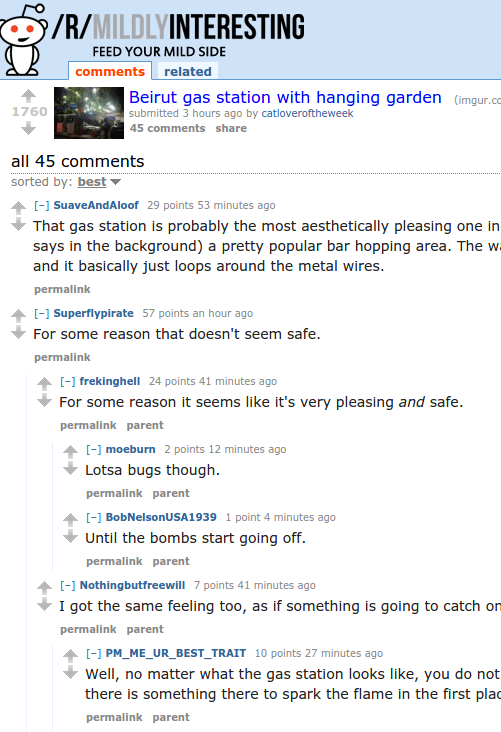
\includegraphics[width=\columnwidth]{reddit-example.png}
\label{fig:reddit-example}
\caption{Example discussion around a Reddit post.}
\end{figure}

The Reddit dataset~\cite{reddit-data} is comprised of a sequence of comments, with one JSON record for each one.
These are ordered temporally.
Reddit itself is roughly similar to a forum, where top-level divisions are made by topic.
Within each topic, or {\em subreddit}, there are posts, which begin with either a short piece of text or a link to an external resource -- typically an image, video, or interesting article.
Users then may publish comments for each post, and reply to each others' comments.
This leads to a threaded discussion, centred on a particular topic, with a hierarchical comment structure (see Figure~\ref{fig:reddit-example}).



NER:

- blended text type approach as in ritter 2011

- CRF w/ classical features and all brown string depth features

- use entity-recognition toolkit

- describe reddit annotation/tuning annotation approach (skim, find things it got wrong, annotate them, add to set)

- estimate Brown c, w based on impact paper findings

- extract reddit tuning set

- tune twitter / newswire balance

- one, three, four, ten entity classes?

- prefer precision? which beta value?




% if have a single appendix:
%\appendix[Proof of the Zonklar Equations]
% or
%\appendix  % for no appendix heading
% do not use \section anymore after \appendix, only \section*
% is possibly needed

% use appendices with more than one appendix
% then use \section to start each appendix
% you must declare a \section before using any
% \subsection or using \label (\appendices by itself
% starts a section numbered zero.)
%


%\appendices
%\section{Proof of the First Zonklar Equation}
%Appendix one text goes here.
%
%% you can choose not to have a title for an appendix
%% if you want by leaving the argument blank
%\section{}
%Appendix two text goes here.
%
%
%% use section* for acknowledgment
%\section*{Acknowledgment}
%
%
%The authors would like to thank...
%
%
%% Can use something like this to put references on a page
%% by themselves when using endfloat and the captionsoff option.
%\ifCLASSOPTIONcaptionsoff
%  \newpage
%\fi



% trigger a \newpage just before the given reference
% number - used to balance the columns on the last page
% adjust value as needed - may need to be readjusted if
% the document is modified later
%\IEEEtriggeratref{8}
% The "triggered" command can be changed if desired:
%\IEEEtriggercmd{\enlargethispage{-5in}}

% references section

% can use a bibliography generated by BibTeX as a .bbl file
% BibTeX documentation can be easily obtained at:
% http://www.ctan.org/tex-archive/biblio/bibtex/contrib/doc/
% The IEEEtran BibTeX style support page is at:
% http://www.michaelshell.org/tex/ieeetran/bibtex/
\bibliographystyle{IEEEtran}
% argument is your BibTeX string definitions and bibliography database(s)
%\bibliography{IEEEabrv,NER-Diffusion}
\bibliography{NER-Diffusion}
%
% <OR> manually copy in the resultant .bbl file
% set second argument of \begin to the number of references
% (used to reserve space for the reference number labels box)
%\begin{thebibliography}{1}
%
%\bibitem{IEEEhowto:kopka}
%H.~Kopka and P.~W. Daly, \emph{A Guide to \LaTeX}, 3rd~ed.\hskip 1em plus
%  0.5em minus 0.4em\relax Harlow, England: Addison-Wesley, 1999.
%
%\end{thebibliography}
%
%% biography section
%% 
%% If you have an EPS/PDF photo (graphicx package needed) extra braces are
%% needed around the contents of the optional argument to biography to prevent
%% the LaTeX parser from getting confused when it sees the complicated
%% \includegraphics command within an optional argument. (You could create
%% your own custom macro containing the \includegraphics command to make things
%% simpler here.)
%%\begin{IEEEbiography}[{\includegraphics[width=1in,height=1.25in,clip,keepaspectratio]{mshell}}]{Michael Shell}
%% or if you just want to reserve a space for a photo:
%
%\begin{IEEEbiography}{Michael Shell}
%Biography text here.
%\end{IEEEbiography}
%
%% if you will not have a photo at all:
%\begin{IEEEbiographynophoto}{John Doe}
%Biography text here.
%\end{IEEEbiographynophoto}
%
%% insert where needed to balance the two columns on the last page with
%% biographies
%%\newpage
%
%\begin{IEEEbiographynophoto}{Jane Doe}
%Biography text here.
%\end{IEEEbiographynophoto}

% You can push biographies down or up by placing
% a \vfill before or after them. The appropriate
% use of \vfill depends on what kind of text is
% on the last page and whether or not the columns
% are being equalized.

%\vfill

% Can be used to pull up biographies so that the bottom of the last one
% is flush with the other column.
%\enlargethispage{-5in}



% that's all folks
\end{document}


